% !TeX spellcheck = en_GB
\chapter{Implementation and Testing} % Realisierung und Test
\epigraph{Any fool can write code that a computer can understand. Good programmers write code that humans can understand.}{Martin Fowler}


\section{Development Setup}\label{sec:development-setup}

Figure~\ref{fig:development-setup} illustrates the development setup in the form of an UML deployment diagram.
A developer connects via his browser to the reverse proxy that serves the \gls{xmpp-grid} \gls{broker} web application.
The HTTP connection from the client to the server is secured using mutual \gls{tls} authentication.
The same reverse proxy also routes the \gls{xmpp} connections.
The client also authenticates to the proxy using mutual \gls{tls} authentication, and the proxy afterwards establishes a \gls{tls} connection to the \gls{xmpp} server using his client certificates.
The reasons for this setup is described in more detail in Section~\fullref{sec:limitations-of-the-openfire-xmpp-server}.

\begin{figure}[h]
    \centering
    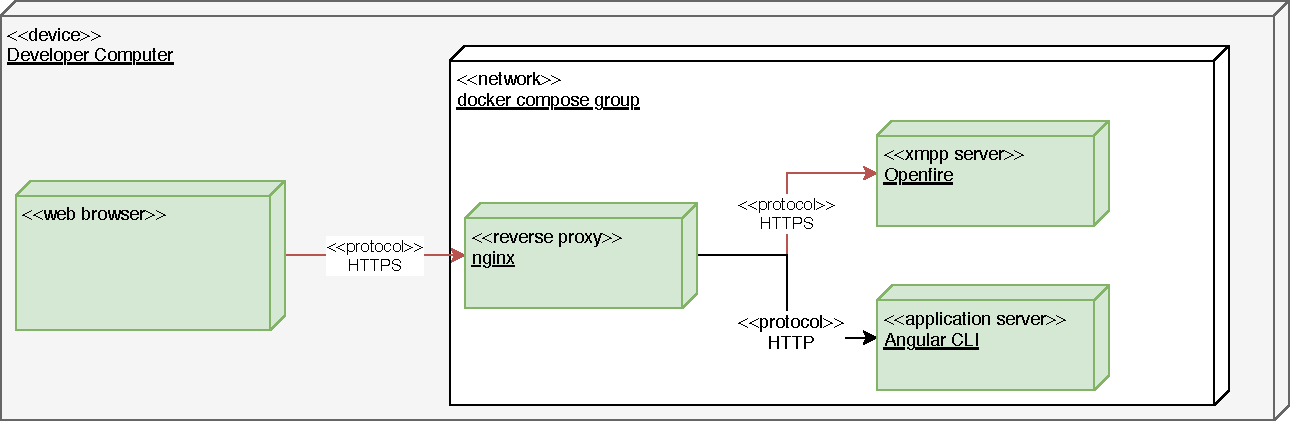
\includegraphics[width=1\linewidth]{resources/development-setup-uml}
    \caption{UML Deployment Diagram presenting the development setup}
    \label{fig:development-setup}
\end{figure}

As the previously described structure is not trivial, the guiding principle for our development setup was to maximise automation and minimise manual setup and configuration efforts. This principle is the basis for a durable software.
We decided on a docker and docker-compose\footnote{\url{https://www.docker.com/}} based stack that provides a correctly configured Openfire instance, a preconfigured nginx\footnote{\url{https://www.nginx.com/}} instance as well as client and server certificates.
Everyday tasks such as generating new certificates or building and testing the application and documentation were automated as bash scripts.

The efforts invested in this docker setup proved valuable when we began to write integration tests that run in the same environment.

We deliberately decided to run unit tests outside of the docker environment as unit tests are executed more often, and the additional docker-overhead would, therefore, be unnecessarily expensive.
Also, debugging is more straightforward without any indirections.

\section{Encountered Problems}\label{encountered-problems}

\subsection{Limitations of \emph{\fullref{sec:requirement-multiple-administrators}}}\label{sec:limitations-of-requirement-multiple-administrators}

Requirement \ref{sec:requirement-multiple-administrators} states that multiple administrators should be able to access the application.

When authenticating users with \gls{sasl-external}, the client certificate extension field `xmppAddr' is interpreted as user \gls{jid} by the \gls{xmpp} server.

In practice, most \gls{xmpp-grid} \gls{broker} deployments will require an HTTP proxy in front of the \gls{xmpp} server as security measure\footnote{
More information on this can be found in Section~\fullref{sec:implemented-web-application-topology}.}.
Usually, the HTTP proxy can also be used to serve the \gls{broker} application.
Such an HTTP proxy might also accept multiple different client certificates.

If the client connects to the \gls{xmpp} server over secure WebSockets (WSS) in combination with \gls{sasl-external}, the WebSocket URL must already be authenticated, as most browsers do not permit certificate selection on background requests\footnote{\url{https://bugs.chromium.org/p/chromium/issues/detail?id=329884\#c24}}.
This might be achieved by serving the \gls{broker} from the same domain or by using client certificate policies\footnote{\url{https://support.google.com/chrome/a/answer/6080885?hl=en\#manage-certs}}.

As the proxy intercepts the \gls{tls} connection, it must verify the client certificate sent by the browser and establish a connection to the \gls{xmpp} server using a client certificate as well.
Therefore, the `xmppAddr' field of the proxy's client ceritifcate is used by the \gls{xmpp} server.
If multiple users should be differentiated on the \gls{xmpp} server, an HTTP proxy might choose different client certificates for connecting to the \gls{xmpp} server based on the web browser's client certificate `xmppAddr'.


\subsection{Limitations of \emph{\fullref{sec:requirement-audit-trail}}}

Actions of administrators should be traceable with an audit trail according to requirement \ref{sec:requirement-audit-trail}.

As outlined in Section~\ref{sec:limitations-of-requirement-multiple-administrators}, practical deployments of \gls{xmpp-grid} \glspl{broker} will mostly use a HTTP proxy.
Additionally, to handling the client authentication, the proxy can be used to keep an audit trail of client requests.
These requests can then be correlated with the query log on the \gls{xmpp} server.

Creating audit trails on the client side does not provide additional safety, as users might prevent trail entries by manipulating the client application.
Therefore, no such mechanism was implemented.

\subsection{Limitations of \emph{\fullref{sec:requirement-logout}}}

Administrators should be able to terminate a session by using a logout function, as stated in requirement~\ref{sec:requirement-logout}.

After evaluating different authentication mechanism in the architectural decision about \gls{sasl} Authentication Strategy (see Appendix~\ref{sec:architectural-decisions}), we decided to use \gls{tls} client certificate authentication (as part of \gls{sasl-external}). In combination with our decision to write a web application, the web browser is responsible for the \gls{tls} authentication.

Unfortunately, web browsers do not expose a standardised way to log out of a \gls{tls} client authenticated session \cite{practical-issues-with-tls-client}.
To close the \gls{tls} session, administrators should close their browser window after using the \gls{xmpp-grid} \gls{broker}.

\subsection{Limitations due to \gls{xmpp} or \gls{xep} Standards}

Multiple shortcomings in the relevant \glspl{xep} were discovered during the realisation of the proposed architecture, that would have lead to a highly inefficient implementation of some requirements and therefore prevented us from implementing them.

\subsubsection{Recursive Listing and Filtering of all \glspl{topic}}

Requirement~\fullref{sec:requirement-list-all-topics} states that an administrator should be able to list all topics recursively.

This requirement could not be implemented efficiently, as the current \gls{publish-subscribe} \gls{xep} does not support direct recursive queries of \glspl{topic}, but only the root level or children of a specific \gls{topic}.

Therefore, we implemented a recursive approach in the client, that queries all \glspl{topic} and recursively requests all child \glspl{topic} to be displayed.

For the same reason, we did not implement requirement~\fullref{sec:requirement-topic-filter} as for a full search, the whole \glspl{topic} tree would have to be traversed on the client side.
With an assumed count of approximately 1000 \glspl{topic}, this would result in large performance overhead.

\subsubsection{Filtering and Paging of \glspl{persisted-item}}

Requirements~\fullref{sec:requirement-filter-persisted-items} and \fullref{sec:paged-persisted-items} were built on the premise that filtering and paging of \glspl{persisted-item} would be possible with the \gls{jabber-search} \cite{xep-0055} and the  \gls{result-set-management} \cite{xep-0059} \glspl{xep}.

Sadly, the \gls{publish-subscribe} \gls{xep} does not define an integration with \gls{jabber-search}.

Retrieving multiple \glspl{persisted-item} in \gls{result-set-management} pages was added in version 1.12 (2008-09-03) only of the \gls{publish-subscribe} \gls{xep}.
A \gls{xmpp} server does not report, which version of the standard it supports.

Therefore, we could not presume an implementation of \gls{result-set-management}.
In fact, the Openfire \gls{xmpp} server we used in our setup has no support for retrieving \glspl{persisted-item} with \gls{result-set-management}. We were still able to fetch the persisted items in pages using \gls{service-discovery}, as the \gls{result-set-management} draft uses service-discovery as an example, making the server side support more likely \cite{xep-0059}.

\subsubsection{Create and Configure \glspl{topic}}

We have four requirements that are concerned with the initial configuration of \glspl{topic}:
\begin{itemize}
  \item \fullref{sec:requirement-topic-default-configuration}
  \item \fullref{sec:requirement-collection-default-configuration}
  \item \fullref{sec:requirement-initial-topic-consumer-provider}
  \item \fullref{sec:requirement-initial-collection-consumer}
\end{itemize}

The implementation of providing initial configuration for a \glspl{topic} is only partially possible due to limitations in the \gls{publish-subscribe} standard. The default configuration can be fetched, but it must it does not necessarily comprise all possible configuration options of a \glspl{topic}.
As managing consumers (via subscriptions) and providers (via consumers) are separate concepts from the configuration an can only be configured after a \gls{topic} has been created, we concluded that a two-step process is more appropriate. ~\cite{xep-0060}

\subsection{Limitations of the Openfire \gls{xmpp} Server}\label{sec:limitations-of-the-openfire-xmpp-server}

As discussed in Section~\ref{sec:development-setup}, the Openfire \gls{xmpp} server was used in the development setup. This section details on the encountered limitations while implementing the \gls{xmpp-grid} \gls{broker}.

\subsubsection{WebSocket \gls{sasl-external} Support}

At the time of this thesis, Openfire does not support \gls{sasl-external} in combination with \gls{xmpp} over WebSockets.
Therefore, the current implementation of the \gls{xmpp-grid} \gls{broker} was developed with \gls{bosh}, but also support communication over WebSockets thanks to the stanza.io \gls{xmpp} library\footnote{\url{https://github.com/legastero/stanza.io}}.

\subsubsection{Lost Updates}\label{sec:lost-updates}

When editing the configuration of a \gls{topic}, Openfire exposes multiple fields that depend on each other.
One example of this is the configuration of how many \glspl{persisted-item} should be kept.
If persisting Items on a \gls{topic} is disabled, openfire does neither update the field nor respond with an error as specified in the standard \cite{xep-0060, xep-0004}.

This behaviour is not user-friendly at all, as an administrator might want to change configuration options pro-actively. To circumvent this problem, a functionality to compare any changes in the new configuration of a topic after storing all changes might be implemented in the future.

\subsubsection{Wrong Field Types}

At time of this writing, Openfire returns wrong \gls{data-forms} field types for some \gls{publish-subscribe} fields.
Although modifing the field type is explicitly allowed by the standard \cite{xep-0060}, the usability of these fields suffer.
A prominent example is the `pubsub\#node\_type' field, which is presented as a text field instead of a limited selection.

A support request at the Openfire~project was opened\footnote{\url{https://discourse.igniterealtime.org/t/wrong-field-type-of-pubsub-node-type-and-how-to-update-it/81596}},
which is mandatory before filing an issue in the Openfire issue tracker.
However, there was no response until the editorial deadline of this thesis.

Should the type of such fields change in the future, the flexible implementation of \gls{data-forms} in our implementation is sufficient to reflect the new form type.

\section{Code Quality}
As our \gls{xmpp-grid} \gls{broker} implementation is intended to be a maintainable, production-ready application rather than a prototype, we placed much emphasis on code quality.
The measures taken can broadly be divided into three categories: technical measures, strategic decisions and processes.

\subsubsection{Technical Measures and Strategic Decisions}
Using Angular and the default Angular CLI was mostly a strategic decision.
Deviating as less as possible from the standard configuration ensures long-term maintainability and relatively straight-forward upgrades to newer Angular versions.
Another benefit of the Angular CLI project setup is that it comes with ``codelyzer''\footnote{\url{http://codelyzer.com/}} (including ``tslint'') for static code analysis and style linting.

Apart from the built-in linting mechanism, we followed Angular's Style Guide~\cite{angular-style-guide}.
Using the JetBrains IDEs (IntelliJ Ultimate and Webstorm)\footnote{\url{https://www.jetbrains.com/}} turned out to be particularly helpful as they give quick feedback for frequent mistakes and even violations of the Angular Style Guide.

We would have prefered to use more tools, especially for code metrics such as Lack of Cohesion of Methods (LCOM), and Afferent/Efferent Coupling.
However, we were not able to find such tools that were actively maintained and work with TypeScript.

\subsubsection{Processes}

On the process side, we tried to work test driven as much as possible.
Doing so turned out to be harder than expected as Angular's component testing infrastructure and the actual calls are sometimes wide apart (see Section~\fullref{sec:testing}).

Another process we heavily relied on were code reviews.
Each change, for the documentation and code, was reviewed using GitHub pull-requests\footnote{\url{https://www.github.com/}}.
In most cases, minor changes were detected and addressed during these reviews.
Continuous integration with TravisCI\footnote{\url{https://travis-ci.com/}} ensured that these changes never contained compilation errors or failing tests.

We also regularly discussed architectural and structural questions in our retrospectives and standup meetings.

In general, writing clean, modular and testable code has been our main priority.

\section{Testing}\label{sec:testing}

Good tests are inevitable for long-lived software projects.
They help developers to ensure that everything (still) works as expected after a change.
For the \gls{xmpp-grid} \gls{broker}, we focused on unit and end-to-end tests.
Following the principles of the test pyramid \cite{Cohn:2009:SAS:1667109}, we wrote many cheap and fast unit tests verifying the fundamental behaviour and fewer expensive and complex end to end tests.

\subsubsection{Unit Tests}

Testing the Angular Services was rather straightforward just by using jasmine and its mocking functionality.
We deliberately abstained from using Angulars testing framework for these services to keep them simple and comprehensible.
However, most of the services mainly send and receive \gls{xmpp}-commands for which integration or end to end tests are required.

Writing tests for Angular Components, which require actual rendering a web browser, was not always essential.
To have fine-grained control and to be able to conduct tests, Angular provides a rather complex set of testing tools.
Because of this indirection, tests are conceptually not identical with the actual Angular application, making test driven development harder if not impossible.

\subsubsection{End to End Tests}

The end-to-end tests were written using Protractor, Angulars official end-to-end testing framework.
Protractor starts the development setup and verifies the application using a remote-controlled browser.

End-to-end tests are usually more challenging to write than unit tests, as different types of race conditions and varying delays to backend applications can occur.
Protractor usually resolves these issue due to its use of Zone.js, a library that creates ``execution context[s] that persists across async tasks'' called Zones.
To create Zones, Zone.js intercepts most web browser events, like HTTP requests.~\cite{zone-js-readme}

Because Zone.js is aware of all open HTTP requests, protractor can wait until a request and document change has completed before continuing with test execution.

However, due to our use of \gls{bosh} in the end-to-end tests\footnote{See Section~\fullref{sec:implemented-web-application-topology}}, we could not benefit from the Zone.js change detection.
\gls{bosh} uses HTTP long polling to communicate with the \gls{xmpp} server, which leads to a Zone that always has open requests~\cite{xep-0124}.

Therefore, we had to manually implement waiting conditions, which proved to be difficult due to unstable behaviour of the application stack in different environments.

In our case, writing tests paid off quickly as they promptly caught many potential bugs introduced by small changes and refactorings.

\section{Documentation}

Install instructions, as well as security best practices, are directly documented in the git source code repository using a plain text file format called AsciiDoc.
Interested parties can browse the documentation directly on GitHub, which is not uncommon in the open source community.

A compact getting started guide for developers is also available in the source code repository.
The source code has jsdoc\footnote{\url{http://usejsdoc.org/}} based documentation optimised for compodoc, a ``documentation tool for your Angular applications''\footnote{\url{https://compodoc.app/}}.

As already discussed in Section \fullref{sec:architecture}, all architectural decisions were documented systematically.
These decisions enable new developers and interested parties to comprehend why certain decisions were made.
With the idea of making project documentation durable, all decisions were written in the same plaintext format as the other project documentation.
